\documentclass{beamer}

\usetheme{default}
\usepackage[utf8]{inputenc}
\usepackage{tikz}
\usepackage{tabularx}
\usetikzlibrary{positioning}
\usepackage{amsmath}


\usepackage{algorithm}
\usepackage{algorithmic}
\usepackage{float}

\setbeamertemplate{footline}[frame number]
\setbeamertemplate{frametitle}[default][center]

\mode<presentation>{
\usetheme{Dresden}
%\setbeamercovered{transparent}
\usecolortheme{seagull}
}

\setbeamertemplate{headline}{}

\definecolor{peeblue}{RGB}{1,123,165}
\setbeamercolor*{palette primary}{fg=black,bg=peeblue!80}
\setbeamercolor*{palette secondary}{fg=black,bg=peeblue!80!gray!80}
\setbeamercolor*{palette tertiary}{fg=black,bg=peeblue!100}
\setbeamercolor*{palette quaternary}{fg=black,bg=peeblue!110}

\usebackgroundtemplate
{%
    \begin{picture}(210,40)(-5,2)
    
\includegraphics[width=0.07\paperwidth,keepaspectratio]{imgs/pee-logo-short.png}
    \end{picture}%
}

 \AtBeginSection[]
  {
    \begin{frame}
      \centering
      \huge\insertsectionhead
    \end{frame}
  }

\title{Técnicas de Regularização em Aprendizado Profundo}
\author{Rickson Monteiro \\ Miguel Fernandes \\ Evandro Rocha   }
\date{\today}

\institute
{
  Universidade Federal do Rio de Janeiro\\
  UFRJ/COPPE/PEE
}


% Let's get started
\begin{document}

{
\usebackgroundtemplate{
    \begin{picture}(210,55)(-5,0)
    
\includegraphics[height=0.14\paperwidth,keepaspectratio]{imgs/pee-logo.png}
    \end{picture}%
    \begin{picture}(210,55)(-28,2)
    
\includegraphics[height=0.14\paperwidth,keepaspectratio]{imgs/coppe-logo.pdf}
    \end{picture}
}
\begin{frame}
  \bigskip\bigskip\bigskip\bigskip
  \titlepage
\end{frame}
}

\begin{frame}{Agenda}
  \tableofcontents
\end{frame}

\section{Introdução}

\begin{frame}{Problema}
\begin{itemize}
  \item Por quê estudar regularização em \textit{deep learning}?
  \item R.: \textit{Overfitting} 
\end{itemize}
\end{frame}

\begin{frame}{Possíveis causas de \textit{Overfitting}}
\begin{itemize}
  \item Complexidade do modelo;
  \item Poucos dados de Treinamento;
  \item Ruídos excessivos nos dados;
  \item Treinamento por tempo excessivo.
\end{itemize}
\end{frame}

\begin{frame}{Formalização matemática}
    \begin{equation*}
        E_{out}(g) \le E_{in}(g) + \sqrt{\frac{8}{\mathcal{N}} \ln \left( \frac{4((2\mathcal{N})^{d_{vc}} + 1)}{\delta} \right)}
    \end{equation*}
    Onde:
    \begin{itemize}
        \item $\mathcal{N}$: Número de exemplos de treinamento (tamanho da amostra).
        \item $\mathcal{H}$: Conjunto de hipóteses (espaço de modelos) que o algoritmo está usando (a complexidade da família de modelos).
        \item $d_{vc}$: Dimensão VC (Vapnik-Chervonenkis). Medida da capacidade/complexidade do espaço de hipóteses $\mathcal{H}$.
    \end{itemize}
\end{frame}

\begin{frame}{Exemplo de Overfitting}
\centering
\includegraphics[width=\textwidth,height=0.8\textheight,keepaspectratio]{imgs/bishop_example/1.png}
\end{frame}

\begin{frame}{Erro x Grau do polinômio}
    \centering
    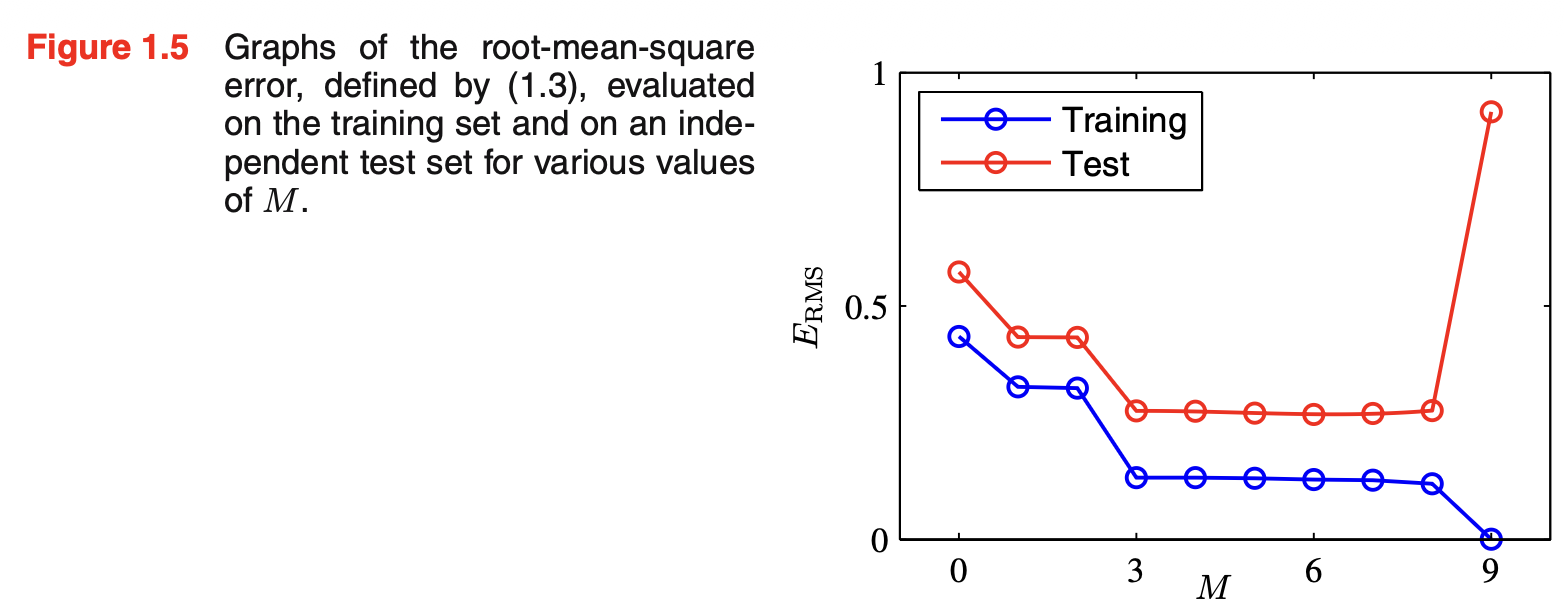
\includegraphics[width=\textwidth,height=0.8\textheight,keepaspectratio]{imgs/bishop_example/2.png}
\end{frame}

\begin{frame}{Possíveis soluções}
    \begin{enumerate}
        \item Aumentar a quantidade de dados de treinamento.
    \end{enumerate}
\end{frame}

\begin{frame}{Alternativa 1: aumentar a quantidade de dados no treinamento}
\tiny{\textit{"The best way to make a machine learning model generalize better is to train it on
more data. Of course, in practice, the amount of data we have is limited."} --- Goodfellow et al., \textit{Deep Learning}}
\centering
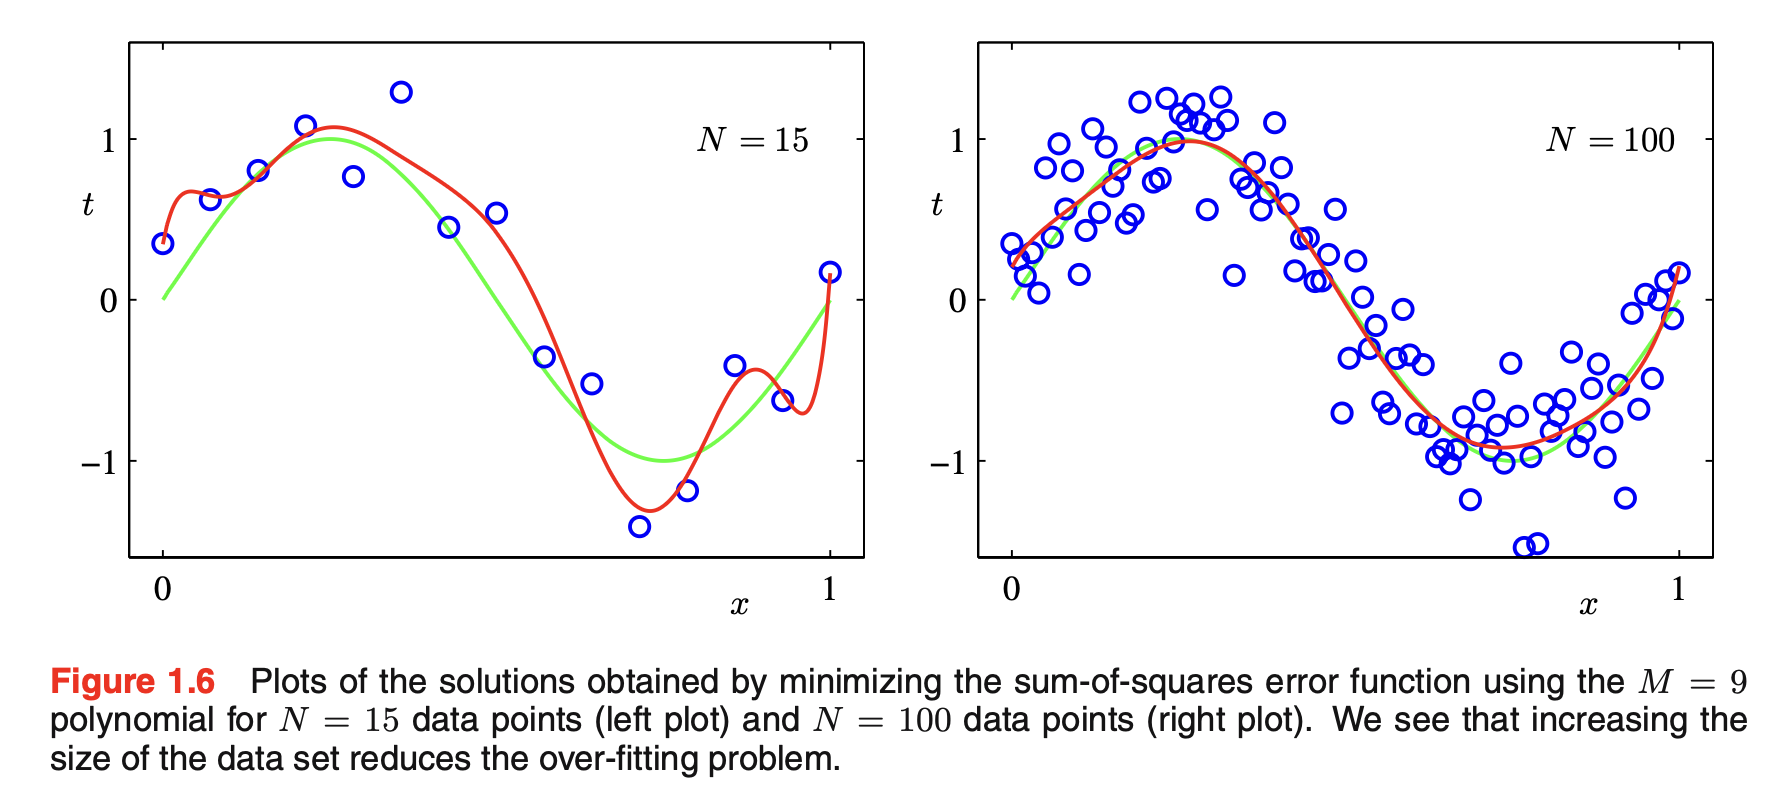
\includegraphics[width=\textwidth,height=0.8\textheight,keepaspectratio]{imgs/bishop_example/3.png}
\end{frame}

\begin{frame}{Possíveis soluções}
    \begin{enumerate}
        \item Aumentar a quantidade de dados de treinamento.
        \item \textbf{Regularização}.
    \end{enumerate}
\end{frame}

\begin{frame}{Definição}
\begin{quote}
``Any modification we make to a learning algorithm that is intended to reduce its generalization error but not its training error.''
\end{quote}
\vspace{0.5cm}
\raggedleft
--- Goodfellow et al. Deep Learning
\end{frame}


\begin{frame}{Alternativa 2: aplicar regularização}
\centering
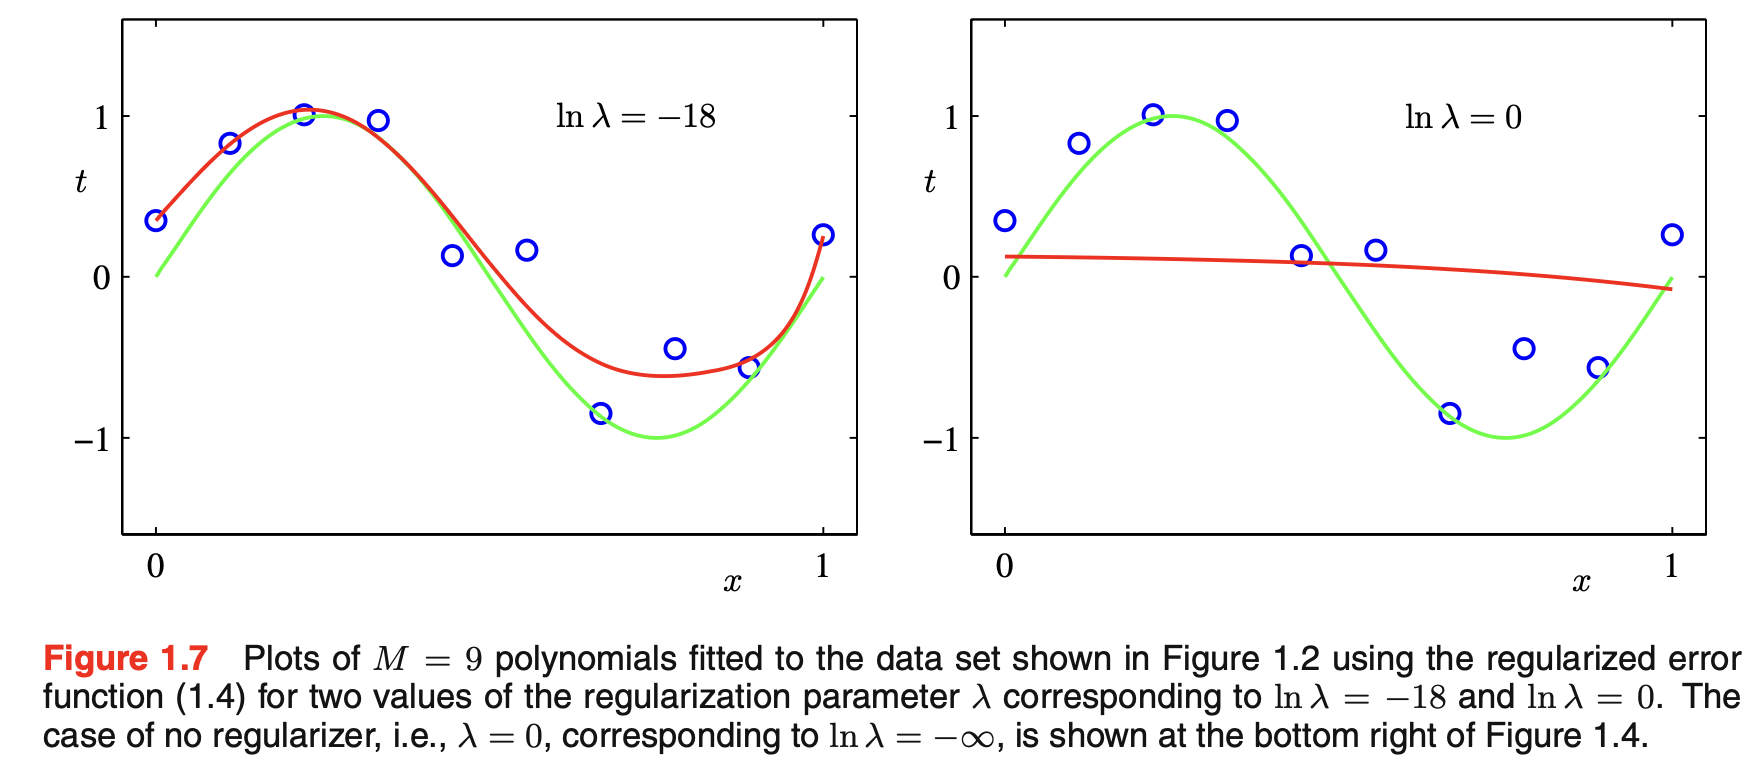
\includegraphics[width=\textwidth,height=0.8\textheight,keepaspectratio]{imgs/bishop_example/4.png}
\end{frame}

\begin{frame}
\centering
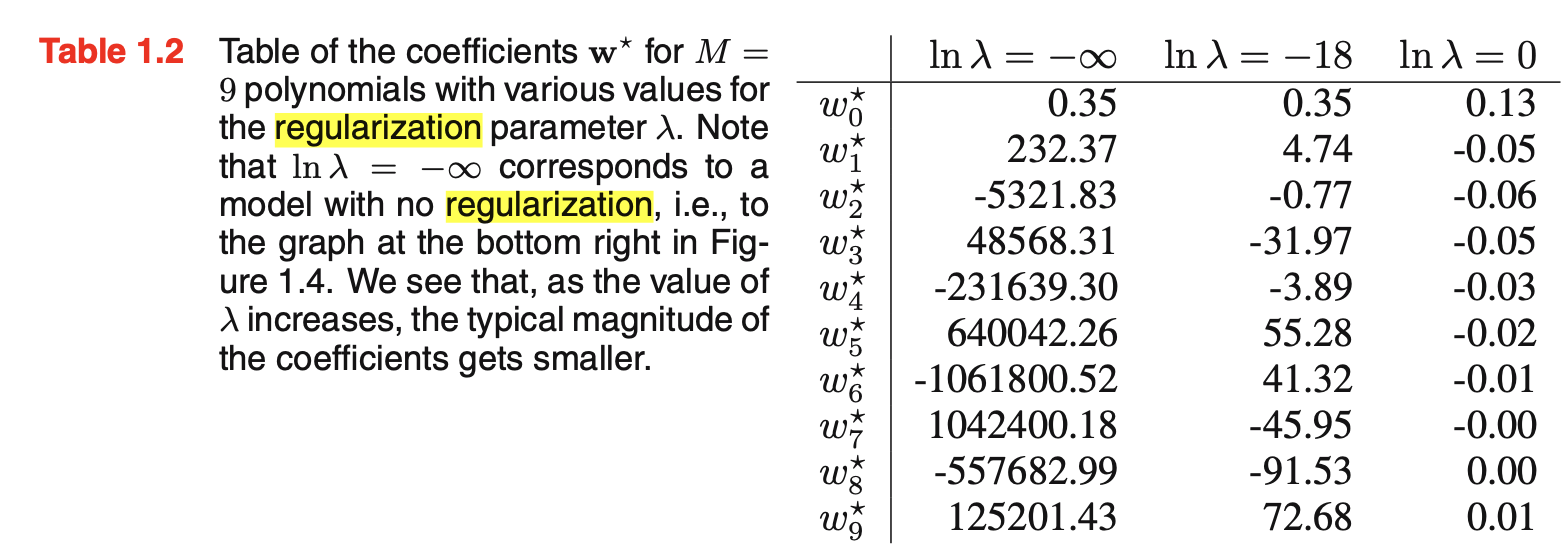
\includegraphics[width=\textwidth,height=0.8\textheight,keepaspectratio]{imgs/bishop_example/5.png}


\footnotesize{
Na prática, o valor de $\lambda$ pode ser validado com o auxílio do procedimento de validação cruzada.}
\end{frame}

\section{Otimização com Restrições}

\begin{frame}{Penalização da Norma dos Parâmetros}
\begin{columns}[T]
\begin{column}{0.5\textwidth}
\begin{block}{Regularização L1}
\vspace{0.2cm}
\scriptsize
\[
\mathcal{L}(\theta) = \frac{1}{N}\sum_{i=1}^{N}\text{Custo}(y_i, f_\theta(x_i)) + \lambda||\theta||_1
\]
\vspace{0.3cm}
\begin{itemize}
    \item Seleção de Variáveis (\textit{Sparsity/Esparsidade})
    \item Redução dos Coeficientes (\textit{Shrinkage/Encolhimento}) a uma taxa constante
\end{itemize}
\vspace{0.2cm}
\end{block}

\end{column}

\begin{column}{0.48\textwidth}
\begin{block}{Regularização L2}
\vspace{0.2cm}
\scriptsize
\[
\mathcal{L}(\theta) = \frac{1}{N}\sum_{i=1}^{N}\text{Custo}(y_i, f_\theta(x_i)) + \lambda||\theta||_2^2
\]
\vspace{0.3cm}
\begin{itemize}
    \item Contribui para a estabilidade numérica
    \item Redução de Coeficientes a uma taxa proporcional (Shrinkage/Encolhimento)
\end{itemize}
\vspace{0.2cm}
\end{block}

\end{column}
\end{columns}
\tiny{\begin{quote}
    \textit{"Regularization terms of the form (above) encourage the model weights to have a smaller magnitude and hence introduce a bias towards functions that vary more slowly with changes in the inputs."} --- Bishop et al., \textit{Deep Learning}
\end{quote}}
\end{frame}


\begin{frame}{Regularização L1 – Gradiente e Shrinkage}
Para um modelo de Regressão Linear, onde a função de perda não regularizada é o Erro Quadrático Médio (MSE), a função de custo regularizada L1, $\mathcal{L}(w)$, é definida por:

\begin{equation}
    \mathcal{L}(w) = \text{MSE}(w) + \lambda \sum_{j=1}^{M} |w_j|
\end{equation}

    \noindent onde:
    \begin{align*}
        w &= (w_1, w_2, \dots, w_M) && \text{Vetor de coeficientes} \\
        \text{MSE}(w) &= \frac{1}{N} \sum_{i=1}^{N} (y^{(i)} - \hat{y}^{(i)})^2 && \text{Erro quadrático médio;} \\
        \lambda &\ge 0 && \text{Intensidade da penalização;} \\
        \sum_{j=1}^{M} |w_j| &= \|w\|_1 && \text{Norma $L_1$ dos coeficientes.}
    \end{align*}
\end{frame}

\begin{frame}{Regularização L1 – Gradiente e Shrinkage}
O objetivo é encontrar o vetor de coeficientes $w^*$ que minimiza a função de custo:
    \begin{equation}
    w^* = \arg\min_{w} \left[ \text{MSE}(w) + \lambda \sum_{j=1}^{M} |w_j| \right]
    \end{equation}
\end{frame}


\begin{frame}{Regularização L1 – Gradiente e Shrinkage}
Analisando a derivada parcial da função de custo em relação a um coeficiente específico $w_j$, obtém-se:

\begin{equation}
\frac{\partial \mathcal{L}(w),}{\partial w_j} = \frac{\partial \, \text{MSE}(w)}{\partial w_j} + \lambda \, \frac{\partial |w_j|}{\partial w_j}
\end{equation}

O termo $\dfrac{\partial \, \text{MSE}(w)}{\partial w_j}$ representa o gradiente da função de perda não regularizada ($g_j$).
\end{frame}



\begin{frame}{Regularização L1 – Gradiente e Shrinkage}
O termo de penalidade tem a derivada:

\begin{equation}
\frac{\partial |w_j|}{\partial w_j} =
\begin{cases}
+1, & \text{se } w_j > 0 \\
-1, & \text{se } w_j < 0 \\
\text{indefinido}, & \text{se } w_j = 0
\end{cases}
= \operatorname{sgn}(w_j), \quad \text{para } w_j \ne 0
\end{equation}

A regra de atualização do coeficiente $w_j$ usando o Gradiente Descendente é (para $w_j \ne 0$):

\begin{equation}
w_j^{\text{novo}} = w_j^{\text{antigo}} - \eta \, \frac{\partial \mathcal{L}(w)}{\partial w_j}
= w_j^{\text{antigo}} - \eta \, (g_j + \lambda \cdot \operatorname{sgn}(w_j^{\text{antigo}}))
\end{equation}

\begin{equation}
w_j^{\text{novo}} = w_j^{\text{antigo}} - \eta \, g_j - \eta \, \lambda \, \operatorname{sgn}(w_j^{\text{antigo}})
\end{equation}
\end{frame}


\begin{frame}{Regularização L1 – Gradiente e Shrinkage}
A solução direta do gradiente é problemática porque 
$\partial \mathcal{L}(w)/\partial w_j$ não é diferenciável em $w_j = 0$. 
Isso significa que os pesos podem não ser zerados exatamente na solução.  

Uma abordagem para contornar isso é usar o conceito de \textbf{subgradiente}, aplicado através da técnica conhecida como \textit{soft-thresholding}, que define cada peso como:

\[
w_j^* =
\begin{cases}
w_j^{OLS} - \frac{\lambda}{Q_j}, & w_j^{OLS} > \frac{\lambda}{Q_j} \\
0, & |w_j^{OLS}| \le \frac{\lambda}{Q_j} \\
w_j^{OLS} + \frac{\lambda}{Q_j}, & w_j^{OLS} < -\frac{\lambda}{Q_j}
\end{cases}
\]

onde $w_j^{OLS}$ é o peso obtido pela regressão linear sem regularização, 
e $Q_j = \sum_i x_{ij}^2$.  

\textbf{A implementação detalhada da técnica de soft-thresholding não será abordada aqui.}
\end{frame}



\begin{frame}{Regularização L2 – Gradiente e Shrinkage}
Para a regularização L2 a função de custo é:

\begin{equation}
\mathcal{L}(w) = \text{MSE}(w) + \lambda \sum_{j=1}^{M} w_j^2
\end{equation}

A derivada parcial em relação a $w_j$ é:

\begin{equation}
\frac{\partial \mathcal{L}(w)}{\partial w_j}
= \frac{\partial \, \text{MSE}(w)}{\partial w_j}
+ \lambda \, \frac{\partial (w_j^2)}{\partial w_j}
= g_j + 2\lambda w_j
\end{equation}

\end{frame}

\begin{frame}{Regularização L2 – Gradiente e Shrinkage}
Logo, a regra de atualização do coeficiente $w_j$ é:

\begin{equation}
w_j^{\text{novo}} = w_j^{\text{antigo}} - \eta \, \frac{\partial \mathcal{L}(w)}{\partial w_j}
\end{equation}

\begin{equation}
w_j^{\text{novo}} = w_j^{\text{antigo}} - \eta g_j - 2\eta\lambda w_j^{\text{antigo}}
\end{equation}
\end{frame}

\begin{frame}{Regularização L2 – Remoção de multicolinearidade}
Além da redução proporcional dos coeficientes, a regularização L2 também contribui para a estabilidade numérica do problema de inversão da matriz $X^TX$ no caso da presença de \textit{features} altamente correlacionadas.


\begin{equation}
\mathcal{L}_{\text{ridge}}(\mathbf{w}) =
\|y - X\mathbf{w}\|_2^2 + \lambda \|\mathbf{w}\|_2^2
\end{equation}

Derivando em relação a $\mathbf{w}$ e igualando a zero:
\begin{equation}
(X^T X + \lambda I)\mathbf{w} = X^T y
\end{equation}

\begin{equation}
    \mathbf{w} = (X^T X + \lambda I)^{-1} X^T y
\end{equation}

\end{frame}





\begin{frame}{L1 x L2}
\scriptsize
\begin{tabularx}{\textwidth}{|l|X|X|}
    \hline
    \textbf{Característica} & \textbf{L1 (Lasso)} & \textbf{L2 (Ridge)} \\ \hline
    Efeito principal & Seleciona variáveis — coeficientes podem ser exatamente zero & Reduz coeficientes proporcionalmente ao peso \\ \hline
    Uso recomendado & Quando se deseja simplificação e seleção automática de variáveis & Quando todas as variáveis são relevantes e deseja-se apenas reduzir variância \\ \hline
    Sparsity (esparsidade) & Sim — tende a gerar muitos coeficientes nulos & Não — tende a manter todos os coeficientes diferentes de zero \\ \hline
    Robustez à multicolinearidade & Baixa — escolhe uma entre variáveis correlacionadas & Alta — distribui pesos entre variáveis correlacionadas de forma estável \\ \hline
\end{tabularx}
\end{frame}






\begin{frame}{Elastic Net}
    \textbf{Fórmula:}
    \[
    \mathcal{L}(\theta) = \frac{1}{N}\sum_{i=1}^{N} \text{Loss}(y_i, f_\theta(x_i)) + \lambda_1 \|\theta\|_1 + \lambda_2 \|\theta\|_2^2
    \]

    \vspace{0.5cm}
    \textbf{Principais características e problemas que resolve:}
    \begin{itemize}
        \item Combina os benefícios do L1 e L2:
        \begin{itemize}
            \item Seleção de variáveis (sparsity) do L1;
            \item Regularização estável e redução de multicolinearidade do L2;
        \end{itemize}
    \end{itemize}
\end{frame}



\begin{frame}{Interpretação Geométrica}
\centering
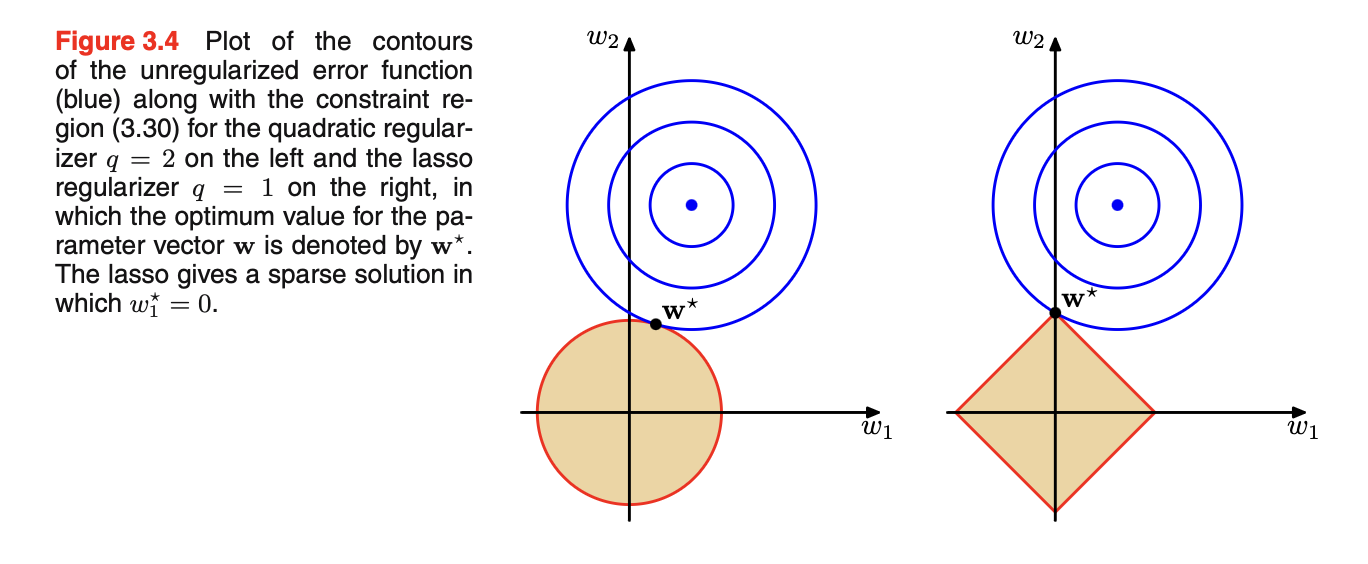
\includegraphics[width=\textwidth,height=0.8\textheight,keepaspectratio]{imgs/bishop_example/7.png}
\end{frame}


\section{Data Augmentation}

\begin{frame}{Aumento de Dados}
\begin{itemize}
  
  \item Em determinadas tarefas, a predição deve ser \textbf{equivariante}. Ex: segmentação em objetos com translação;

  \item Em outras, a predição deve ser \textbf{invariante} a uma ou mais transformações nos dados de entrada: translação, tamanho, rotação, \textbf{ruído}, etc.
\end{itemize}
\end{frame}

\begin{frame}{Aumento de Dados}
Formas de tornar o modelo invariante a transformações:
    \begin{itemize}
      \item Pre-processamento: gerar \textit{features} invariantes às transformações (Ex. Histograma, FFT);
      \item Regularização: penaliza alterações na saída do modelo para uma mesma entrada com as transformações aplicadas;
      \item Modificar a estrutura da rede;
      \item \textbf{Aumentar o conjunto de dados de treinamento}.
    \end{itemize}
\end{frame}


\begin{frame}{Invariância}
\centering
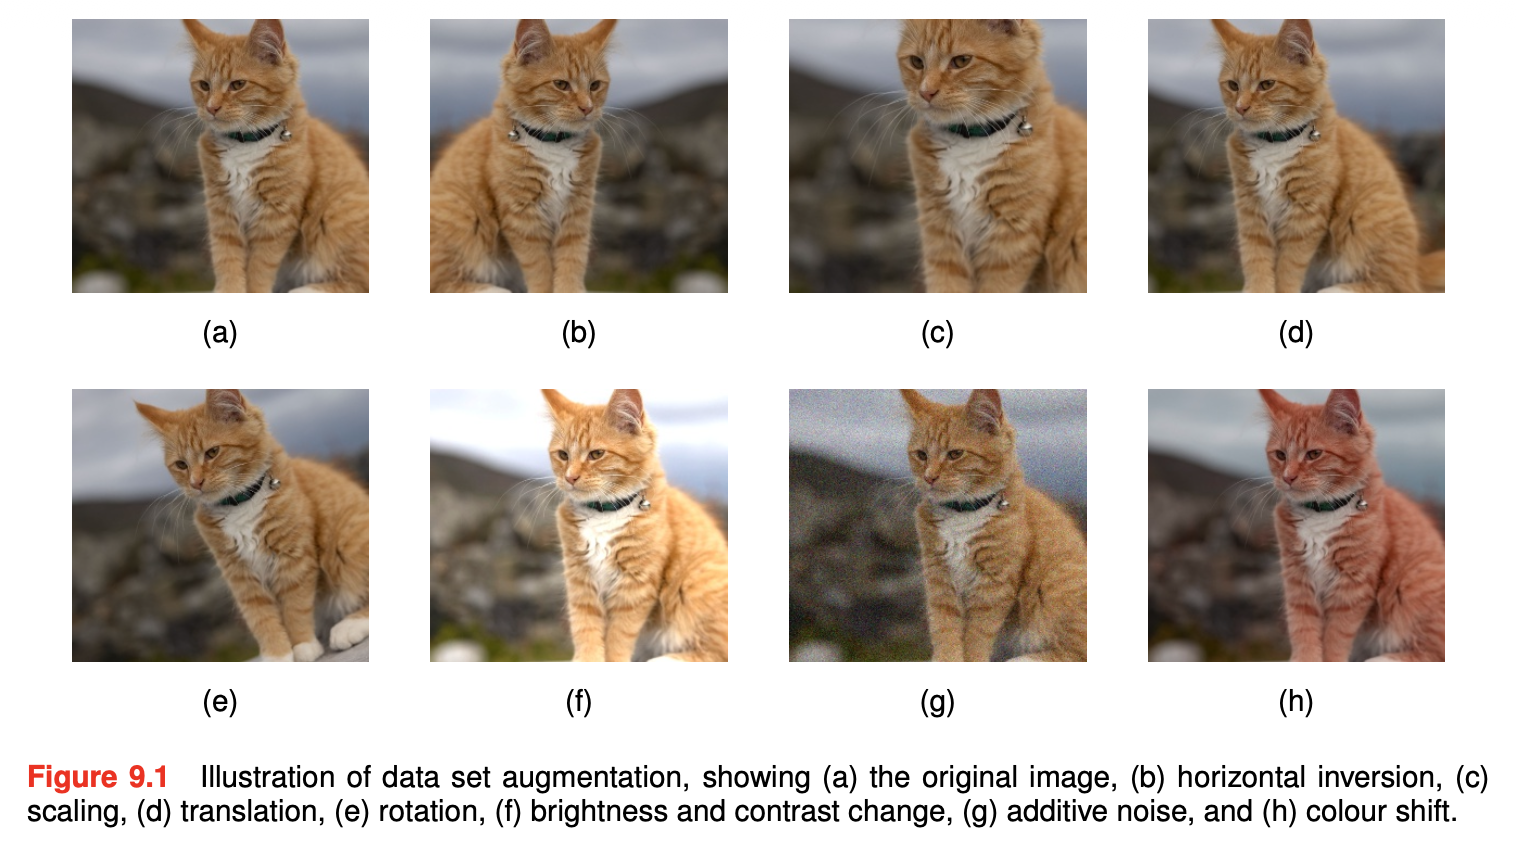
\includegraphics[width=\textwidth,height=0.5\textheight,keepaspectratio]{imgs/bishop_example/8.png}
\begin{itemize}
  \item Reconhecimento de imagem 
\item OCR: cuidado (b e d, 6 e 9)
\end{itemize}
\end{frame}


\begin{frame}{Equivariância}
\centering
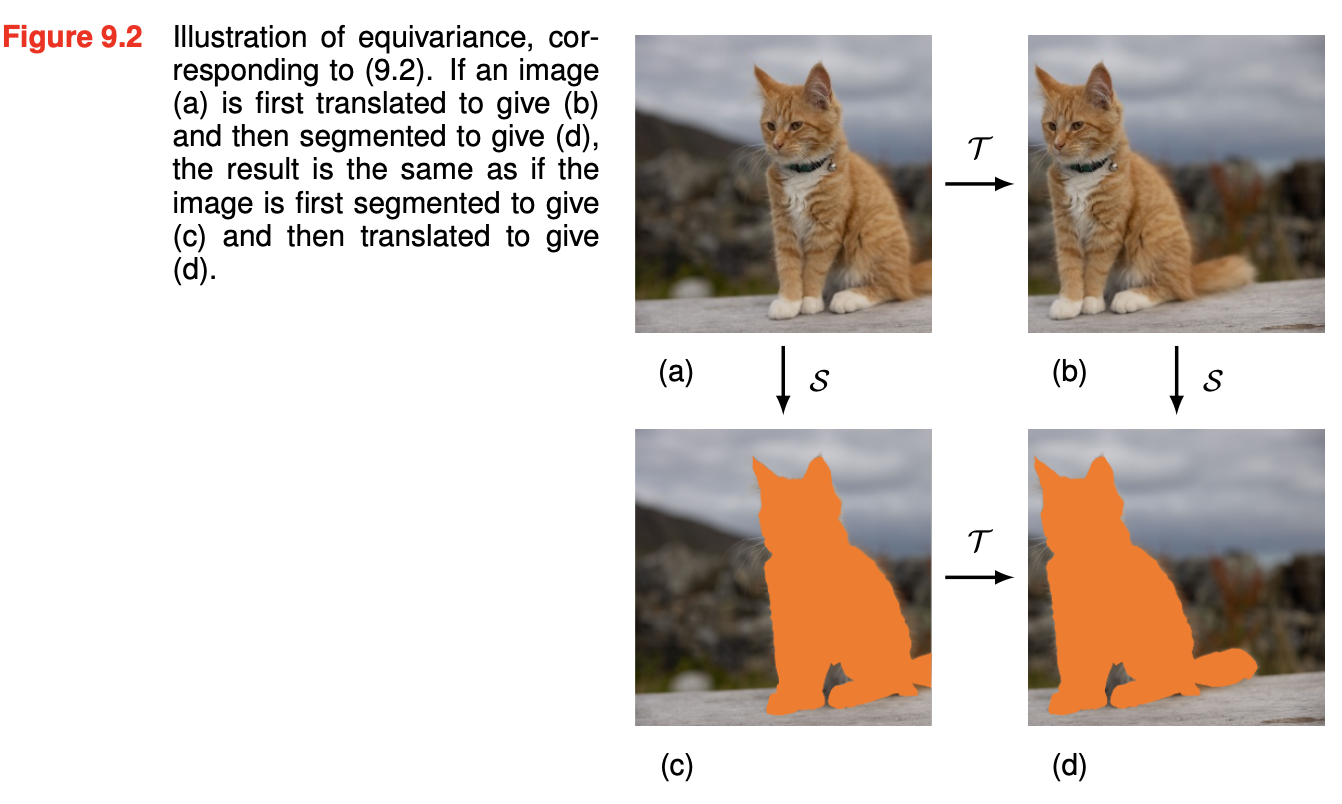
\includegraphics[width=\textwidth,height=0.7\textheight,keepaspectratio]{imgs/bishop_example/9.png}
\end{frame}


\section{Curvas de Aprendizado}
\begin{frame}{Encerramento Antecipado (\textit{Early stopping})}
\begin{figure}[H]
    \centering
    \includegraphics[width=\textwidth,height=0.5\textheight,keepaspectratio]{imgs/goodfellow_example/1.png}
    \caption{Erro de log-verossimilhança em função da quantidade de épocas de treinamento. Rede maxout treinada com dataset MNIST. Retirado de Goodfellow et al., \textit{Deep Learning}.}
\end{figure}
Encaramos o ``tempo de treinamento'' como um hiperparâmetro.
\end{frame}


\begin{frame}{Encerramento Antecipado (\textit{Early stopping})}
  \begin{itemize}
    \item Regularização menos intrusiva.
    \item ``Hiperparâmetro especial'' por ser obtido em uma única execução do treinamento.
    \item O maior custo computacional seria o cálculo do erro para o conjunto de validação, mas pode ser assíncrono.
  \end{itemize}
\end{frame}

\begin{frame}{Encerramento Antecipado (\textit{Early stopping})}
\begin{algorithm}[H]
% \caption{Early stopping meta-algorithm for determining the best amount of time to train}
\tiny
\begin{algorithmic}[1]
\STATE Let $n$ be the number of steps between evaluations.
\STATE Let $p$ be the ``patience,'' the number of times to observe worsening validation set error before giving up.
\STATE Let $\theta_0$ be the initial parameters.
\STATE $\theta \leftarrow \theta_0$
\STATE $i \leftarrow 0$
\STATE $j \leftarrow 0$
\STATE $v \leftarrow \infty$
\STATE $\theta^\ast \leftarrow \theta$
\STATE $i^\ast \leftarrow i$
\WHILE{$j < p$}
    \STATE Update $\theta$ by running the training algorithm for $n$ steps.
    \STATE $i \leftarrow i + n$
    \STATE $v' \leftarrow \text{ValidationSetError}(\theta)$
    \IF{$v' < v$}
        \STATE $j \leftarrow 0$
        \STATE $\theta^\ast \leftarrow \theta$
        \STATE $i^\ast \leftarrow i$
        \STATE $v \leftarrow v'$
    \ELSE
        \STATE $j \leftarrow j + 1$
    \ENDIF
\ENDWHILE
\STATE \textbf{Return} best parameters $\theta^\ast$ and best number of training steps $i^\ast$.
\end{algorithmic}
\end{algorithm}
\end{frame}


\begin{frame}{Encerramento Antecipado (\textit{Early stopping})}
  Após encontrar os melhores parâmetros, há duas estratégias possíveis para o treinamento:
  \begin{itemize}
    \item Reiniciar os pesos do modelo e treinar do zero até a quantidade ``ótima'' de passos;
    \item Manter os pesos do ponto ótimo e continuar o treinamento com todos os dados (treinamento + validação).
    \begin{itemize}
        \item Perde-se a referência da quantidade de passos,
        \item Mas evita o custo de reiniciar o treinamento.
    \end{itemize}
  \end{itemize}
\end{frame}


\begin{frame}{Convenção ``clássica'': compromisso viés-variância}
Assumimos que os dados são gerados por uma função $f(x)$ tal que
\[
y = f(x) + \varepsilon,
\]
onde o ruído $\varepsilon$ tem média zero e variância $\sigma^{2}$.
Assim,
\[
y_{i} = f(x_{i}) + \varepsilon_{i},
\]
onde $\varepsilon_{i}$ é uma amostra de ruído.
\end{frame}
\begin{frame}{Convenção ``clássica'': compromisso viés-variância}
Queremos encontrar uma função $\hat{f}(x; D)$ que aproxime a função verdadeira $f(x)$ tanto quanto possível
\[
D = \{(x_{1}, y_{1}), \dots, (x_{n}, y_{n})\}.
\]
Ou seja, minimizar o erro quadrático médio entre $y$ e $\hat{f}(x; D)$ para os pontos de treinamento $x_{1}, \dots, x_{n}$ e para pontos fora do conjunto de treinamento.

Por conveniência, omite-se o subscrito $D$, tal que $\hat{f}(x; D) = \hat{f}(x)$.

\end{frame}


\begin{frame}{Convenção ``clássica'': compromisso viés-variância}
Por conveniência, omite-se o subscrito $D$, tal que $\hat{f}(x; D) = \hat{f}(x)$.

Define-se o erro quadrático médio (MSE) do modelo como
\begin{align*}
\mathrm{MSE} 
&\triangleq \mathbb{E}\!\left[(y - \hat{f}(x))^{2}\right] \\
&= \mathbb{E}\!\left[(f(x) + \varepsilon - \hat{f}(x))^{2}\right] 
\qquad \text{dado que } y \triangleq f(x) + \varepsilon \\
&= \mathbb{E}\!\left[(f(x) - \hat{f}(x))^{2}\right]
   + 2\,\mathbb{E}\!\left[(f(x) - \hat{f}(x))\,\varepsilon\right]
   + \mathbb{E}\!\left[\varepsilon^{2}\right].
\end{align*}

O segundo termo da equação é zero:
\begin{align*}
\mathbb{E}\!\left[(f(x) - \hat{f}(x))\,\varepsilon\right]
&= \mathbb{E}\!\left[f(x) - \hat{f}(x)\right] \,
   \mathbb{E}\!\left[\varepsilon\right]
   && \text{$\varepsilon$ é independente de $x$} \\
&= 0
   && \text{uma vez que } \mathbb{E}\!\left[\varepsilon\right] = 0.
\end{align*}
\end{frame}

\begin{frame}{Convenção ``clássica'': compromisso viés-variância}
O terceiro termo da equação anterior é a variância do ruído:
\[
\mathbb{E}[\varepsilon^{2}] = \sigma^{2}.
\]

Expandindo o termo restante:
\begin{align*}
\mathbb{E}\!\left[(f(x) - \hat{f}(x))^{2}\right]
&= \mathbb{E}\!\left[
    \big(
        f(x) - \mathbb{E}[\hat{f}(x)]
        + \mathbb{E}[\hat{f}(x)] - \hat{f}(x)
    \big)^{2}
\right] \\[1ex]
&= 
\mathbb{E}\!\left[
    \big(f(x) - \mathbb{E}[\hat{f}(x)]\big)^{2}
\right]
+ 
\mathbb{E}\!\left[
    \big(\mathbb{E}[\hat{f}(x)] - \hat{f}(x)\big)^{2}
\right] \nonumber \\[0.5ex]
&\quad + 2\,\mathbb{E}\!\left[
    \big(f(x) - \mathbb{E}[\hat{f}(x)]\big)
    \big(\mathbb{E}[\hat{f}(x)] - \hat{f}(x)\big)
\right].
\end{align*}
\end{frame}


\begin{frame}{Convenção ``clássica'': compromisso viés-variância}
Uma vez que $f(x)$ não é uma variável aleatória, mas uma função determinística de $x$:
\begin{align*}
\mathbb{E}\!\left[\big(f(x) - \mathbb{E}[\hat{f}(x)]\big)^{2}\right]
&= \mathbb{E}\!\left[f(x)^{2}\right]
   - 2\,\mathbb{E}\!\left[f(x)\,\mathbb{E}[\hat{f}(x)]\right]
   + \mathbb{E}\!\left[\mathbb{E}[\hat{f}(x)]^{2}\right] \\[1ex]
&= f(x)^{2}
   - 2\,f(x)\,\mathbb{E}[\hat{f}(x)]
   + \big(\mathbb{E}[\hat{f}(x)]\big)^{2} \\[1ex]
&= \big(f(x) - \mathbb{E}[\hat{f}(x)]\big)^{2}.
\end{align*}
\end{frame}


\begin{frame}{Convenção ``clássica'': compromisso viés-variância}
Pelo mesmo raciocínio, podemos expandir o termo cruzado e demonstrar que é igual a zero:
\begin{flalign*}
  & \mathbb{E}\!\left[
      \big(f(x) - \mathbb{E}[\hat{f}(x)]\big)
      \big(\mathbb{E}[\hat{f}(x)] - \hat{f}(x)\big)
  \right] && \\
  & = \mathbb{E}\!\left[
      f(x)\,\mathbb{E}[\hat{f}(x)]
      - f(x)\,\hat{f}(x)
      - \big(\mathbb{E}[\hat{f}(x)]\big)^{2}
      + \mathbb{E}[\hat{f}(x)]\,\hat{f}(x)
  \right] && \\[1ex]
  & = f(x)\,\mathbb{E}[\hat{f}(x)]
     - f(x)\,\mathbb{E}[\hat{f}(x)]
     - \big(\mathbb{E}[\hat{f}(x)]\big)^{2}
     + \big(\mathbb{E}[\hat{f}(x)]\big)^{2} && \\[1ex]
  & = 0. &&
  \end{flalign*}
\end{frame}



\begin{frame}{Convenção ``clássica'': compromisso viés-variância}
  Finalmente:
\begin{align}
\mathrm{MSE}
&= \big(f(x) - \mathbb{E_D}[\hat{f}(x)]\big)^{2}
+ \mathbb{E_D}\!\left[\big(\mathbb{E_D}[\hat{f}(x)] - \hat{f}(x)\big)^{2}\right]
+ \sigma^{2} \\[1ex]
&= \operatorname{Bias}\!\left[\hat{f}(x)\right]^{2}
+ \operatorname{Var}\!\left[\hat{f}(x)\right]
+ \sigma^{2}.
\end{align}

A função de custo do erro quadrático médio 
é obtida a partir do valor esperado em relação ao espaço de entradas $X$:
\begin{equation}
\mathrm{MSE}
= \mathbb{E}_{x}\!\left\{
    \operatorname{Bias}_{D}\!\left[\hat{f}(x; D)\right]^{2}
    + \operatorname{Var}_{D}\!\left[\hat{f}(x; D)\right]
\right\}
+ \sigma^{2}.
\end{equation}
\end{frame}

\begin{frame}{Convenção ``clássica'': compromisso viés-variância}
\includegraphics[width=\textwidth,height=0.8\textheight,keepaspectratio]{imgs/bishop_example/113.png}
\end{frame}

\begin{frame}{Convenção ``clássica'': compromisso viés-variância}
\includegraphics[width=\textwidth,height=0.6\textheight,keepaspectratio]{imgs/bishop_example/114.png}

\textbf{Crença clássica:} número de parâmetros deve ser limitado ao tamanho do conjunto de dados
\end{frame}

\begin{frame}{Convenção ``moderna'': \textbf{Double Descent}} 
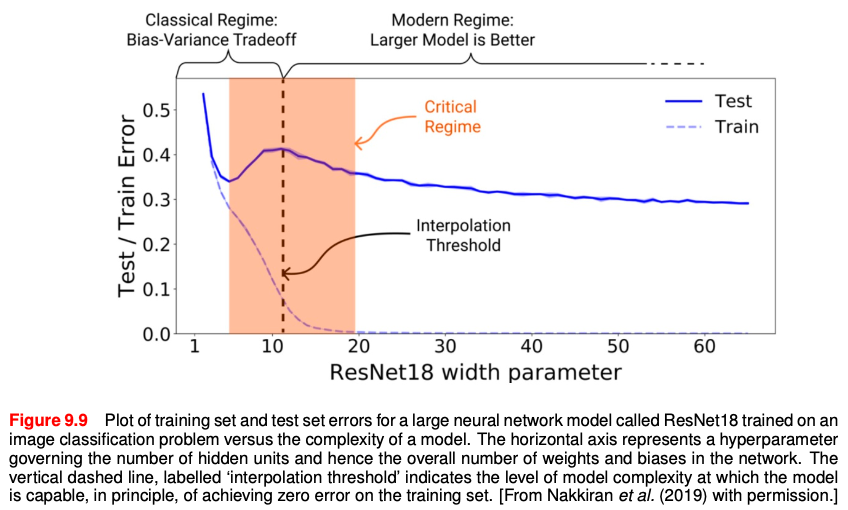
\includegraphics[width=\textwidth,height=0.7\textheight,keepaspectratio]{imgs/bishop_example/11.png}
  \begin{itemize}
  \item \textbf{Redes profundas:} bom desempenho mesmo quando a quantidade de parâmetros excede em muito o necessário para ajustar aos dados de treinamento 
\end{itemize}
\end{frame}

\begin{frame}{Convenção ``moderna'': \textbf{Double Descent}} 
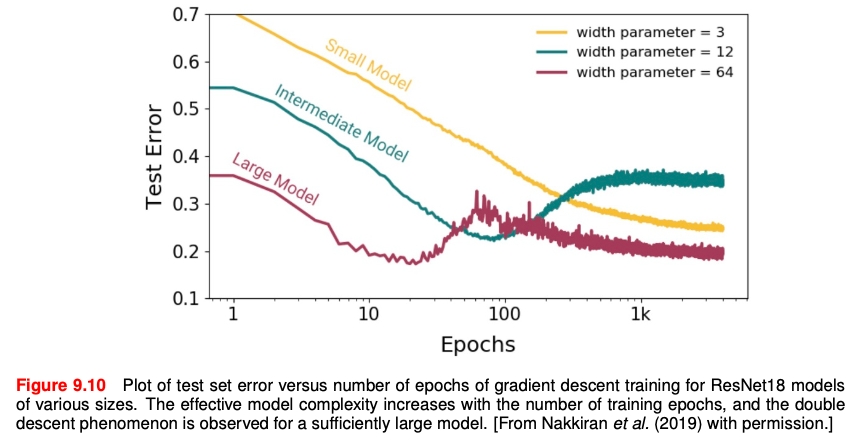
\includegraphics[width=\textwidth,height=0.8\textheight,keepaspectratio]{imgs/bishop_example/12.png}
    \tiny{Complexidade efetiva do modelo: quantidade máxima de dados de treinamento tal que o modelo atinja erro zero (limiar de interpolação). Dali em diante, a descendência dupla ocorre quando a complexidade do modelo excede esse limiar.}
\end{frame}

\section{Dropout}

\begin{frame}{Dropout - Motivação}
\begin{itemize}
    \item \textbf{Problema}: Redes neurais profundas sofrem com \textit{overfitting}
    \item \textbf{Causa}: Co-adaptação excessiva entre neurônios
    \item \textbf{Solução}: Durante o treinamento, ``desligar'' aleatoriamente alguns neurônios
\end{itemize}

\vspace{0.5cm}

\begin{block}{Intuição}
Força a rede a não depender demais de neurônios específicos, criando representações mais robustas
\end{block}

\vspace{0.3cm}
\tiny{Srivastava et al. ``Dropout: A Simple Way to Prevent Neural Networks from Overfitting'' (2014)} 
\end{frame}

\begin{frame}{Dropout - Como Funciona}
\begin{columns}[T]
\begin{column}{0.48\textwidth}
\textbf{Treinamento:}
\begin{itemize}
    \item Para cada iteração:
    \begin{itemize}
        \item Gerar máscara binária aleatória
        \item $m_i \sim \text{Bernoulli}(p)$
        \item Aplicar: $h_i = m_i \cdot a_i$
    \end{itemize}
    \item Taxa de dropout $p$: prob. de manter neurônio
\end{itemize}
\end{column}

\begin{column}{0.48\textwidth}
\textbf{Teste/Inferência:}
\begin{itemize}
    \item Usar todos os neurônios
    \item Escalar saídas por $p$:
    \item $h_i = p \cdot a_i$
\end{itemize}

\end{column}
\end{columns}
\end{frame}

\begin{frame}{Exemplo Visual: Implementação do Dropout}
\centering
\begin{tikzpicture}[scale=0.8, every node/.style={scale=0.8}]
  % Definir posições das camadas
  \def\inputy{3}
  \def\hiddeny{3}
  \def\outputy{1}
  
  % Camada de entrada (3 neurônios)
  \foreach \i in {1,2,3} {
    \node[circle,draw,fill=blue!30,minimum size=0.8cm] (I\i) at (0,\inputy-\i+1) {};
    \node at (I\i) {\scriptsize $x_\i$};
  }
  \node[below] at (0,-0.5) {\small Entrada};
  
  % Primeira camada escondida (4 neurônios)
  \foreach \i in {1,2,3,4} {
    \node[circle,draw,fill=green!30,minimum size=0.6cm] (H1\i) at (2.5,\hiddeny+0.5-\i*0.8) {};
  }
  \node[below] at (2.5,-0.5) {\small Hidden 1};
  
  % Segunda camada escondida (4 neurônios)
  \foreach \i in {1,2,3,4} {
    \node[circle,draw,fill=green!30,minimum size=0.6cm] (H2\i) at (5,\hiddeny+0.5-\i*0.8) {};
  }
  \node[below] at (5,-0.5) {\small Hidden 2};
  
  % Camada de saída (2 neurônios)
  \foreach \i in {1,2} {
    \node[circle,draw,fill=red!30,minimum size=0.6cm] (O\i) at (7.5,\outputy+0.5-\i*0.8) {};
  }
  \node[below] at (7.5,-0.5) {\small Saída};
  
  % Conexões da entrada para primeira camada escondida
  \foreach \i in {1,2,3} {
    \foreach \j in {1,2,3,4} {
      \draw[black, thin] (I\i) -- (H1\j);
    }
  }
  
  % Conexões da primeira para segunda camada escondida
  \foreach \i in {1,2,3,4} {
    \foreach \j in {1,2,3,4} {
      \draw[black, thin] (H1\i) -- (H2\j);
    }
  }
  
  % Conexões da segunda camada escondida para saída
  \foreach \i in {1,2,3,4} {
    \foreach \j in {1,2} {
      \draw[black, thin] (H2\i) -- (O\j);
    }
  }
  
  % Aplicar dropout na primeira iteração (alguns neurônios desligados)
  \only<2>{
    % Desligar neurônios 2 e 4 da primeira camada
    \node[circle,draw,fill=black,minimum size=0.6cm,opacity=0.7] at (2.5,\hiddeny+0.5-2*0.8) {\scriptsize X};
    \node[circle,draw,fill=black,minimum size=0.6cm,opacity=0.7] at (2.5,\hiddeny+0.5-4*0.8) {\scriptsize X};
    
    % Desligar neurônios 1 e 3 da segunda camada
    \node[circle,draw,fill=black,minimum size=0.6cm,opacity=0.7] at (5,\hiddeny+0.5-1*0.8) {\scriptsize X};
    \node[circle,draw,fill=black,minimum size=0.6cm,opacity=0.7] at (5,\hiddeny+0.5-3*0.8) {\scriptsize X};
    
    \node[above] at (3.75, 4) {\textcolor{red}{\textbf{Batch 1: $p = 0.5$}}};
  }
  
  % Aplicar dropout na segunda iteração (diferentes neurônios desligados)
  \only<3>{
    % Desligar neurônios 1 e 3 da primeira camada
    \node[circle,draw,fill=black,minimum size=0.6cm,opacity=0.7] at (2.5,\hiddeny+0.5-1*0.8) {\scriptsize X};
    \node[circle,draw,fill=black,minimum size=0.6cm,opacity=0.7] at (2.5,\hiddeny+0.5-3*0.8) {\scriptsize X};
    
    % Desligar neurônios 2 e 4 da segunda camada
    \node[circle,draw,fill=black,minimum size=0.6cm,opacity=0.7] at (5,\hiddeny+0.5-2*0.8) {\scriptsize X};
    \node[circle,draw,fill=black,minimum size=0.6cm,opacity=0.7] at (5,\hiddeny+0.5-4*0.8) {\scriptsize X};
    
    \node[above] at (3.75, 4) {\textcolor{red}{\textbf{Batch 2: Nova máscara aleatória}}};
  }
  
  % Fase de teste (todos neurônios ativos)
  \only<4>{
    \node[above] at (3.75, 4) {\textcolor{blue}{\textbf{Teste: Todos neurônios ativos (escalados por $p$)}}};
  }
  
\end{tikzpicture}
\end{frame}

\begin{frame}{Dropout - Implementação Matemática}
\begin{columns}[T]
\begin{column}{0.5\textwidth}
\vspace{0.4cm}
\begin{block}{Durante o Treinamento}
\[
\mathbf{r} \sim \text{Bernoulli}(p)
\]
\[
\tilde{\mathbf{x}} = \mathbf{r} \odot \mathbf{x}
\]
\[
\mathbf{y} = W\tilde{\mathbf{x}} + \mathbf{b}
\]
\end{block}

\begin{block}{Durante o Teste}
\[
\mathbf{y} = W(p\mathbf{x}) + \mathbf{b}
\]
\end{block}
\end{column}

\begin{column}{0.48\textwidth}
\small
\textbf{Notação:}
\begin{itemize}
    \item $\mathbf{r}$: máscaras binárias
    \item $\mathbf{x}$: entrada (input)
    \item $\tilde{\mathbf{x}}$: entrada com dropout
    \item $\mathbf{y}$: saída (output)
    \item $W$: matriz de pesos da camada
    \item $\mathbf{b}$: vetor de bias
    \item $\odot$: produto elemento a elemento
    \item $p$: prob. manter neurônio
\end{itemize}

\textbf{Por que $p\mathbf{x}$ no teste?}\\
Compensar diferença de escala: no treinamento só $p$ dos neurônios estão ativos.
\end{column}
\end{columns}
\end{frame}

% Novo slide: Explicação da matriz W
\begin{frame}{Dropout - O que é a Matriz $W$?}
\begin{columns}[T]
\begin{column}{0.48\textwidth}
\textbf{A matriz $W$ contém os pesos da camada:}
\vspace{0.2cm}

Se temos:
\begin{itemize}
    \item Entrada $\mathbf{x}$: 3 elementos
    \item Saída $\mathbf{y}$: 2 elementos
\end{itemize}

Então $W$ é uma matriz $2 \times 3$:
\[
W = \begin{bmatrix} 
w_{11} & w_{12} & w_{13} \\
w_{21} & w_{22} & w_{23}
\end{bmatrix}
\]

Cada $w_{ij}$ conecta o elemento $j$ da entrada ao elemento $i$ da saída.
\end{column}

\begin{column}{0.48\textwidth}
\textbf{Cálculo da saída:}
\[
\mathbf{y} = W\mathbf{x} + \mathbf{b}
\]

\textbf{Exemplo:} Se $W$ é $2 \times 3$:
{\small
\[
W = \begin{bmatrix} 
0.5 & -0.2 & 0.8 \\
0.3 & 0.7 & -0.1
\end{bmatrix}
\]
}

\textbf{Com dropout no teste:}
\[
\mathbf{y} = W(p\mathbf{x}) + \mathbf{b}
\]

Primeiro: $p\mathbf{x}$, depois: $W \times (p\mathbf{x})$.
\end{column}
\end{columns}
\end{frame}

% Novo slide: Explicação detalhada da implementação matemática
\begin{frame}{Dropout - Explicação da Implementação}
\textbf{Passo a passo da implementação:}
\vspace{0.3cm}

\begin{enumerate}
    \item \textbf{Gerar máscaras aleatórias}: Para cada neurônio, sorteia-se um valor binário (0 ou 1) com probabilidade $p$ de ser 1
    \item \textbf{Aplicar máscaras}: Multiplica-se cada ativação pela máscara correspondente (neurônios com máscara 0 são "desligados")
    \item \textbf{Propagar adiante}: Usa-se as ativações modificadas para calcular a saída da camada
    \item \textbf{Durante o teste}: Não há dropout, mas multiplica-se as ativações por $p$ para compensar a diferença de escala
\end{enumerate}

\vspace{0.3cm}
\textbf{Por que funciona?}
\begin{itemize}
    \item Força a rede a não depender de neurônios específicos
    \item Cria um efeito de ensemble implícito (várias subredes diferentes)
    \item Reduz co-adaptação entre neurônios
\end{itemize}
\end{frame}

% Novo slide: Exemplo prático de Dropout
\begin{frame}{Dropout - Exemplo Prático}
\textbf{Exemplo numérico:}
\vspace{0.2cm}

Suponha uma camada com entrada $\mathbf{x} = [0.2, 0.5, 0.8, 0.3]$ e $p = 0.5$.

\vspace{0.2cm}
\textbf{Durante o treinamento:}
\begin{itemize}
    \item Sorteamos $\mathbf{r} \sim \text{Bernoulli}(0.5)$, por exemplo $\mathbf{r} = [1, 0, 1, 0]$
    \item Aplicando o dropout: $\tilde{\mathbf{x}} = \mathbf{r} \odot \mathbf{x} = [0.2, 0, 0.8, 0]$
    \item O cálculo da saída: $\mathbf{y} = W\tilde{\mathbf{x}} + \mathbf{b}$
\end{itemize}

\vspace{0.2cm}
\textbf{Durante o teste:}
\begin{itemize}
    \item Compensamos a escala: $\mathbf{y} = W(p\mathbf{x}) + \mathbf{b} = W([0.1, 0.25, 0.4, 0.15]) + \mathbf{b}$
\end{itemize}

\vspace{0.2cm}
\textbf{Interpretação:} No treinamento, os neurônios 2 e 4 foram ``desligados'', forçando a rede a usar apenas os neurônios 1 e 3.
\end{frame}

\begin{frame}{Dropout - Vantagens e Limitações}
\begin{columns}[T]
\begin{column}{0.48\textwidth}
\textbf{Vantagens:}
\begin{itemize}
    \item Simples de implementar
    \item Muito eficaz contra overfitting
    \item Compatível com diversas arquiteturas
    \item Baixo custo computacional
\end{itemize}
\end{column}

\begin{column}{0.48\textwidth}
\textbf{Limitações:}
\begin{itemize}
    \item Pode tornar treinamento mais lento
    \item Menos eficaz em redes muito profundas
\end{itemize}
\end{column}
\end{columns}

\vspace{0.2cm}
\footnotesize
\begin{block}{Dica Prática}
\begin{itemize}
    \item Começar com $p = 0.5$ para camadas ocultas
    \item $p = 0.8$ para camada de entrada
    \item Ajustar baseado na performance de validação
\end{itemize}
\end{block}
\end{frame}

% Novo slide: Variações do Dropout
\begin{frame}{Dropout - Variações e Extensões}
\begin{columns}[T]
\begin{column}{0.48\textwidth}
\textbf{Inverted Dropout:}
\begin{itemize}
    \item \textbf{Treinamento}: $h_i = \frac{m_i \cdot a_i}{p}$
    \item \textbf{Teste}: $h_i = a_i$ (sem scaling)
    \item \textbf{Vantagem}: Não precisa ajustar no teste
    \item \textbf{Uso}: Implementação mais simples
\end{itemize}

\vspace{0.2cm}
\textbf{DropConnect:}
\begin{itemize}
    \item Remove conexões (pesos) ao invés de neurônios
    \item $r_{ij} \sim \text{Bernoulli}(p)$
    \item $\tilde{W}_{ij} = r_{ij} \cdot W_{ij}$
    \item Mais granular que dropout tradicional
\end{itemize}
\end{column}

\begin{column}{0.48\textwidth}
\textbf{Spatial Dropout:}
\begin{itemize}
    \item Para CNNs: remove feature maps inteiros
    \item Evita correlação espacial
    \item Melhor para dados com estrutura espacial
\end{itemize}

\vspace{0.3cm}
\textbf{Gaussian Dropout:}
\begin{itemize}
    \item Usa ruído gaussiano ao invés de máscaras binárias
    \item $h_i = a_i \cdot \mathcal{N}(1, \sigma^2)$
    \item Transição mais suave
\end{itemize}


\end{column}
\end{columns}
\end{frame}

\section{Batch Normalization}

\begin{frame}{Batch Normalization - Motivação}
\begin{itemize}
    \item \textbf{Problema}: Internal Covariate Shift
    \begin{itemize}
        \item Distribuição das ativações muda durante o treinamento
        \item Cada camada precisa se adaptar às mudanças das camadas anteriores
        \item Torna o treinamento mais lento e instável
    \end{itemize}
    \item \textbf{Solução}: Normalizar as entradas de cada camada
    \item \textbf{Benefícios}:
    \begin{itemize}
        \item Treinamento mais rápido e estável
        \item Permite learning rates maiores
        \item Reduz dependência da inicialização
        \item Efeito regularizador (reduz overfitting)
    \end{itemize}
\end{itemize}

\vspace{0.3cm}
\tiny{Ioffe \& Szegedy ``Batch Normalization: Accelerating Deep Network Training by Reducing Internal Covariate Shift'' (2015)}
\end{frame}

\begin{frame}{Batch Normalization - Como Funciona}
\begin{block}{Algoritmo (para um mini-batch)}
Para cada feature $i$ no mini-batch $\mathcal{B} = \{x_1, x_2, ..., x_m\}$:

\vspace{0.3cm}
1. \textbf{Calcular média}: $\mu_{\mathcal{B}} = \frac{1}{m}\sum_{k=1}^{m} x_k$

2. \textbf{Calcular variância}: $\sigma^2_{\mathcal{B}} = \frac{1}{m}\sum_{k=1}^{m} (x_k - \mu_{\mathcal{B}})^2$

3. \textbf{Normalizar}: $\hat{x}_k = \frac{x_k - \mu_{\mathcal{B}}}{\sqrt{\sigma^2_{\mathcal{B}} + \epsilon}}$

4. \textbf{Escalar e deslocar}: $y_k = \gamma \hat{x}_k + \beta$
\end{block}

\vspace{0.3cm}
Onde:
\begin{itemize}
    \item $\gamma, \beta$: parâmetros aprendíveis (scale e shift)
    \item $\epsilon$: pequena constante para estabilidade numérica ($\sim 10^{-5}$)
\end{itemize}

\vspace{0.3cm}
\textbf{Importância de $\gamma$ e $\beta$:}
\begin{itemize}
    \item Permitem que a rede desfaça a normalização se necessário
    \item $\gamma = \sigma_{\mathcal{B}}$ e $\beta = \mu_{\mathcal{B}}$ recuperam a distribuição original
    \item Inicializados como $\gamma = 1$ e $\beta = 0$
\end{itemize}
\end{frame}

\begin{frame}{Exemplo Visual: Batch Normalization}

\begin{columns}[T]
\begin{column}{0.48\textwidth}
\textbf{Entrada (Mini-batch):}
\vspace{0.3cm}

\begin{tabular}{|c|c|c|}
\hline
\textbf{x1} & \textbf{x2} & \textbf{x3} \\
\hline
2.1 & 0.8 & -1.2 \\
1.8 & 1.1 & -0.9 \\
2.3 & 0.9 & -1.1 \\
1.9 & 1.0 & -1.0 \\
\hline
\end{tabular}

\vspace{0.5cm}
\textbf{Cálculos por feature:}
\begin{itemize}
    \item $\mu_1 = 2.0, \sigma_1 = 0.22$
    \item $\mu_2 = 0.95, \sigma_2 = 0.12$  
    \item $\mu_3 = -1.05, \sigma_3 = 0.12$
\end{itemize}
\end{column}

\begin{column}{0.48\textwidth}
\textbf{Após Normalização:}
\vspace{0.3cm}

\begin{tabular}{|c|c|c|}
\hline
\textbf{$\hat{x}_1$} & \textbf{$\hat{x}_2$} & \textbf{$\hat{x}_3$} \\
\hline
0.45 & -1.22 & -1.22 \\
-0.89 & 1.22 & 1.22 \\
1.34 & -0.41 & -0.41 \\
-0.45 & 0.41 & 0.41 \\
\hline
\end{tabular}

\vspace{0.3cm}
\small Cada coluna agora tem: $\mu = 0$, $\sigma = 1$

\vspace{0.5cm}
\textbf{Saída Final:}
$$y = \gamma \hat{x} + \beta$$
onde $\gamma$ e $\beta$ são aprendidos
\end{column}
\end{columns}

\end{frame}

\begin{frame}{Batch Normalization - Fluxo do Processo}
\centering

\Large
\textbf{Sequência de Transformações:}

\vspace{1cm}

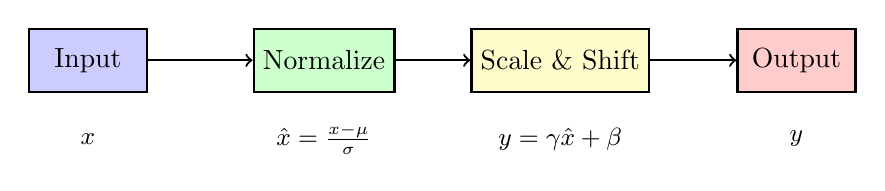
\begin{tikzpicture}
  % Nodes with absolute positioning
  \node[rectangle, draw, thick, fill=blue!20, minimum width=1.5cm, minimum height=0.8cm] (input) at (0,0) {Input};
  \node[rectangle, draw, thick, fill=green!20, minimum width=1.5cm, minimum height=0.8cm] (normalize) at (3,0) {Normalize};
  \node[rectangle, draw, thick, fill=yellow!20, minimum width=1.5cm, minimum height=0.8cm] (scale) at (6,0) {Scale \& Shift};
  \node[rectangle, draw, thick, fill=red!20, minimum width=1.5cm, minimum height=0.8cm] (output) at (9,0) {Output};
  
  % Arrows
  \draw[->, thick] (input) -- (normalize);
  \draw[->, thick] (normalize) -- (scale);
  \draw[->, thick] (scale) -- (output);
  
  % Labels with absolute positioning
  \node at (0,-1) {\small $x$};
  \node at (3,-1) {\small $\hat{x} = \frac{x-\mu}{\sigma}$};
  \node at (6,-1) {\small $y = \gamma\hat{x} + \beta$};
  \node at (9,-1) {\small $y$};
\end{tikzpicture}

\vspace{0.3cm}

\begin{block}{Resumo}
\footnotesize
\begin{itemize}
    \item \textbf{Normalizar}: Centra e padroniza os dados ($\mu=0, \sigma=1$)
    \item \textbf{Escalar \& Deslocar}: Permite à rede aprender a distribuição ideal
    \item \textbf{Parâmetros}: $\gamma$ (escala) e $\beta$ (deslocamento) são treináveis
\end{itemize}
\end{block}
\end{frame}

\begin{frame}{Batch Normalization - Posicionamento}

\textbf{Posição Padrão (Ioffe \& Szegedy):}
\begin{itemize}
    \item Antes da função de ativação
    \item $y = f(BN(Wx + b))$
    \item \textbf{Mais comum na prática}
\end{itemize}

\vspace{0.3cm}
\textbf{Posição Alternativa:}
\begin{itemize}
    \item Após a função de ativação
    \item $y = BN(f(Wx + b))$
    \item Menos utilizada
\end{itemize}

\end{frame}

\begin{frame}{Batch Normalization -  Representação visual}
\centering
\textbf{Exemplo: Rede com Batch Normalization}

\vspace{0.5cm}

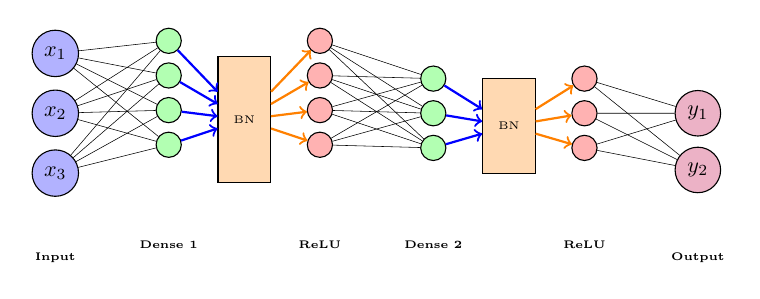
\begin{tikzpicture}[scale=0.80, every node/.style={scale=0.80}]
  % Input layer
  \foreach \i in {1,2,3} {
    \node[circle,draw,fill=blue!30,minimum size=0.5cm] (I\i) at (0,3.5-\i*0.95) {$x_\i$};
  }
  \node[below] at (0,-0.5) {\tiny \textbf{Input}};
  
  % Hidden Layer 1
  \foreach \i in {1,2,3,4} {
    \node[circle,draw,fill=green!30,minimum size=0.4cm] (H1\i) at (1.8,3.3-\i*0.55) {};
  }
  \node[below] at (1.8,-0.3) {\tiny \textbf{Dense 1}};
  
  % Batch Norm 1
  \node[rectangle,draw,fill=orange!30,minimum width=0.7cm,minimum height=2cm,text width=0.6cm,align=center] (BN1) at (3,1.5) {\tiny BN};
  
  % Activation 1
  \foreach \i in {1,2,3,4} {
    \node[circle,draw,fill=red!30,minimum size=0.4cm] (A1\i) at (4.2,3.3-\i*0.55) {};
  }
  \node[below] at (4.2,-0.3) {\tiny \textbf{ReLU}};
  
  % Hidden Layer 2
  \foreach \i in {1,2,3} {
    \node[circle,draw,fill=green!30,minimum size=0.4cm] (H2\i) at (6,2.7-\i*0.55) {};
  }
  \node[below] at (6,-0.3) {\tiny \textbf{Dense 2}};
  
  % Batch Norm 2
  \node[rectangle,draw,fill=orange!30,minimum width=0.7cm,minimum height=1.5cm,text width=0.6cm,align=center] (BN2) at (7.2,1.4) {\tiny BN};
  
  % Activation 2
  \foreach \i in {1,2,3} {
    \node[circle,draw,fill=red!30,minimum size=0.4cm] (A2\i) at (8.4,2.7-\i*0.55) {};
  }
  \node[below] at (8.4,-0.3) {\tiny \textbf{ReLU}};
  
  % Output layer
  \foreach \i in {1,2} {
    \node[circle,draw,fill=purple!30,minimum size=0.5cm] (O\i) at (10.2,2.5-\i*0.9) {$y_\i$};
  }
  \node[below] at (10.2,-0.5) {\tiny \textbf{Output}};
  
  % Connections Input -> Hidden 1
  \foreach \i in {1,2,3} {
    \foreach \j in {1,2,3,4} {
      \draw[black, very thin] (I\i) -- (H1\j);
    }
  }
  
  % Connections Hidden 1 -> BatchNorm 1
  \foreach \i in {1,2,3,4} {
    \draw[->, thick, blue] (H1\i) -- (BN1);
  }
  
  % Connections BatchNorm 1 -> Activation 1
  \foreach \i in {1,2,3,4} {
    \draw[->, thick, orange] (BN1) -- (A1\i);
  }
  
  % Connections Activation 1 -> Hidden 2
  \foreach \i in {1,2,3,4} {
    \foreach \j in {1,2,3} {
      \draw[black, very thin] (A1\i) -- (H2\j);
    }
  }
  
  % Connections Hidden 2 -> BatchNorm 2
  \foreach \i in {1,2,3} {
    \draw[->, thick, blue] (H2\i) -- (BN2);
  }
  
  % Connections BatchNorm 2 -> Activation 2
  \foreach \i in {1,2,3} {
    \draw[->, thick, orange] (BN2) -- (A2\i);
  }
  
  % Connections Activation 2 -> Output
  \foreach \i in {1,2,3} {
    \foreach \j in {1,2} {
      \draw[black, very thin] (A2\i) -- (O\j);
    }
  }
  
\end{tikzpicture}

\vspace{0.3cm}
\footnotesize
\textbf{Fluxo:} Input → Dense → \textcolor{orange}{BatchNorm} → ReLU → Dense → \textcolor{orange}{BatchNorm} → ReLU → Output
\end{frame}


\begin{frame}{Batch Normalization - Vantagens e Limitações}
\begin{columns}[T]
\begin{column}{0.48\textwidth}
\textbf{Vantagens:}
\begin{itemize}
    \item Acelera convergência significativamente
    \item Permite learning rates maiores
    \item Menos sensível à inicialização
    \item Evita overfitting (efeito regularizador)
    \item Reduz gradient vanishing
    \item Amplamente suportado
\end{itemize}
\end{column}

\begin{column}{0.48\textwidth}
\textbf{Limitações:}
\begin{itemize}
    \item Problemas com batch size pequeno
    \item Custo computacional adicional
    \item Memória extra para estatísticas
\end{itemize}
\end{column}
\end{columns}

\vspace{0.5cm}

\end{frame}


\begin{frame}{Alternativas ao Batch Normalization}
\begin{itemize}
    \item \textbf{Layer Normalization}: 
    \begin{itemize}
        \item Normaliza ao longo das features (eixo das características)
        \item Independe do tamanho do batch
        \item Muito útil para RNNs e Transformers
    \end{itemize}
    
    \item \textbf{Group Normalization}: 
    \begin{itemize}
        \item Divide features em grupos e normaliza cada grupo
        \item Intermediário entre Layer e Instance Normalization
        \item Eficaz para CNNs com batch pequeno
    \end{itemize}
    
    \item \textbf{Instance Normalization}: 
    \begin{itemize}
        \item Normaliza cada amostra independentemente
        \item Útil para transferência de estilo em imagens
        \item Preserva contraste entre amostras
    \end{itemize}
\end{itemize}
\end{frame}

\section{Combinação de Técnicas de Regularização}
% --- Introdução à Combinação de Técnicas ---
\begin{frame}{Combinação de Técnicas de Regularização}
\begin{itemize}
  \item Em problemas reais, uma única técnica de regularização pode não ser suficiente para evitar overfitting.
  \item É comum e recomendado combinar diferentes técnicas para potencializar o efeito regularizador.
  \item Combinações bem escolhidas podem melhorar a generalização e a robustez do modelo.
  \item A escolha das técnicas depende do problema, arquitetura e dados disponíveis.
\end{itemize}
\end{frame}

% --- Combinação de Técnicas de Regularização ---
\begin{frame}{Por que combinar técnicas de regularização?}
\begin{itemize}
  \item Cada técnica atua de forma diferente para reduzir o overfitting:
  \begin{itemize}
    \item L1/L2 controlam a magnitude dos pesos
    \item Dropout força a rede a não depender de neurônios específicos
    \item Batch Normalization estabiliza o treinamento, acelerando a convergência
    \item Data Augmentation aumenta a diversidade dos dados
  \end{itemize}
  \item Combinar técnicas potencializa a regularização e cobre diferentes fontes de overfitting
  \item Prática comum em redes profundas modernas
  \item Pode melhorar robustez e generalização sem grande aumento de custo computacional
\end{itemize}
\end{frame}

\begin{frame}{Exemplos de combinações}
\scriptsize
\begin{itemize}
  \item \textbf{EfficientNet (Tan \& Le, 2019):}
  \begin{itemize}
    \item Data Augmentation + Batch Norm + Dropout + L2
    \item AutoAugment para melhor generalização em CNNs
  \end{itemize}
  
  \item \textbf{DenseNet (Huang et al., 2017):}
  \begin{itemize}
    \item Batch Norm + Dropout + L2 + Data Augmentation
    \item Conexões densas para melhor fluxo de gradientes
  \end{itemize}
  
  \item \textbf{Show and Tell (Vinyals et al., 2015):}
  \begin{itemize}
    \item Early Stopping + Dropout + L2 + Data Augmentation
    \item Image captioning com CNN + LSTM
  \end{itemize}
  
  \item \textbf{AWD-LSTM (Merity et al., 2017):}
  \begin{itemize}
    \item Dropout + L2 + DropConnect
    \item Regularização agressiva para modelagem de linguagem
  \end{itemize}
   \item \textbf{Recomendações:}
  \begin{itemize}
    \item Testar diferentes combinações, monitorando validação
    \item Cuidado com excesso: regularização demais pode prejudicar o aprendizado
  \end{itemize}
\end{itemize}
\end{frame}

\section{Conclusão}
\begin{frame}{Resumo das Técnicas de Regularização}
\begin{itemize}
    \item \textbf{Regularização é fundamental} para evitar overfitting em deep learning
    
    \item \textbf{Múltiplas abordagens complementares:}
    \begin{itemize}
        \item \textbf{Penalização}: L1, L2
        \item \textbf{Estrutural}: Dropout
    \item \textbf{Dados}: Data Augmentation
    \item \textbf{Critério de Parada}: Early Stopping
        \item \textbf{Normalizações}: Batch Normalization
    \end{itemize}
    
    \item \textbf{Cada técnica tem suas características:}
    \begin{itemize}
        \item \textbf{L1/L2}: Simples, sempre aplicável
        \item \textbf{Dropout}: Eficaz para fully-connected layers (camadas totalmente conectadas)
  \item \textbf{Batch Normalization}: Normaliza as ativações, acelera o treinamento (permite taxas de aprendizado maiores) e atua como regularizador (dificulta o overfitting)
    \end{itemize}
\end{itemize}
\end{frame}

\begin{frame}{Conclusões e Recomendações}
\begin{itemize}
    \item \textbf{Escolha da técnica} depende do contexto:
    \begin{itemize}
        \item \textbf{Tipo de dados}: imagem, texto, tabular
        \item \textbf{Arquitetura}: CNN, RNN, Transformer
        \item \textbf{Recursos}: tamanho do dataset, batch size, tempo
    \end{itemize}
    
    \item \textbf{Podemos combinar técnicas} para melhores resultados:
    \begin{itemize}
        \item L2 + Dropout + Batch Norm (combinação clássica)
        \item Data Augmentation + técnicas estruturais
    \end{itemize}
    
    \item \textbf{Regularização bem aplicada} = melhor generalização e modelos mais robustos (menos sensível a ruídos e variações)
\end{itemize}

\end{frame}

\begin{frame}{Referências}
\footnotesize
\begin{itemize}
    \item \textbf{Goodfellow, I., Bengio, Y., \& Courville, A.} (2016). \textit{Deep Learning}. MIT Press. Disponível em: \url{https://www.deeplearningbook.org/}
    
    \item \textbf{Bishop, C. M.} (2006). \textit{Pattern Recognition and Machine Learning}. Springer.
    
    \item \textbf{Srivastava, N., Hinton, G., Krizhevsky, A., Sutskever, I., \& Salakhutdinov, R.} (2014). Dropout: A Simple Way to Prevent Neural Networks from Overfitting. \textit{Journal of Machine Learning Research}, 15, 1929-1958.
    
    \item \textbf{Ioffe, S., \& Szegedy, C.} (2015). Batch Normalization: Accelerating Deep Network Training by Reducing Internal Covariate Shift. \textit{ICML 2015}.
    
    \item \textbf{He, K., Zhang, X., Ren, S., \& Sun, J.} (2016). Deep Residual Learning for Image Recognition. \textit{CVPR 2016}.
\end{itemize}
\end{frame}

\begin{frame}{Referências}
\footnotesize
\begin{itemize}
    \item \textbf{Tan, M., \& Le, Q. V.} (2019). EfficientNet: Rethinking Model Scaling for Convolutional Neural Networks. \textit{ICML 2019}.
    
    \item \textbf{Huang, G., et al.} (2017). Densely Connected Convolutional Networks. \textit{CVPR 2017}.
    
    \item \textbf{Vinyals, O., et al.} (2015). Show and Tell: A Neural Image Caption Generator. \textit{CVPR 2015}.
    
    \item \textbf{Merity, S., et al.} (2017). Regularizing and Optimizing LSTM Language Models. \textit{arXiv:1708.02182}.
    
    \item \textbf{Ng, A.} (2016). Machine Learning Yearning. Disponível em: \url{https://www.mlyearning.org/}
\end{itemize}
\end{frame}

\begin{frame}{Perguntas}
\centering
\Large
\textbf{Perguntas?}

\vspace{1cm}

\end{frame}

\end{document}
